\documentclass[a4paper,12pt]{article} 

\usepackage[unicode, pdftex]{hyperref}
\usepackage{caption}
\usepackage{subcaption}

%Добавляет возможность искать и копировать текст
\usepackage{cmap}

%Убирает пробел между названием таблицы/рисунка и самой таблицей/рисунком
\usepackage{caption}
\captionsetup[table]{skip= -0 cm}
\captionsetup[figure]{skip= -0 cm}

%Выравнивание названия таблиц по левому краю
%\usepackage[nooneline]{caption} 
%Размеры отступов 
\usepackage[left=20mm, top=20mm, right=20mm, bottom=20mm, footskip=10mm]{geometry}

%Рисунки
\usepackage{graphicx}
\usepackage{wrapfig} %обтекание элементов
\graphicspath{{graphs}{figures}}  % папки с картинками

%Русский язык в формулах
\usepackage{mathtext}

%  Русский язык
\usepackage[T2A]{fontenc}			
\usepackage[utf8]{inputenc}			
\usepackage[english,russian]{babel}	

%Красная строка для первого абзаца
\usepackage{indentfirst}

%Готические буквы
\usepackage{amssymb}

% Математика
\usepackage{amsmath,amsfonts,amssymb,amsthm,mathtools} 
\usepackage{wasysym}

%Цветные подписи в таблице
\usepackage[table,xcdraw]{xcolor}

\usepackage{fancyhdr} % Колонтитулы
 	\pagestyle{fancy}
 	\renewcommand{\headrulewidth}{0.3mm}  % Толщина линейки, отчеркивающей верхний колонтитул
 	%\lfoot{Нижний левый}
 	%\rfoot{Нижний правый}
 	\rhead{Белостоцкий Артмемий, Б04-006}
 	%\chead{Верхний в центре}
 	\lhead{Лабораторная работа №9.1}
 	\renewcommand{\footrulewidth}{0.3mm}
 	\cfoot{\thepage} % По умолчанию здесь номер страницы
 	
 	
%\captionsetup[table]{
%  position=above,
%  justification=raggedright,
  %labelsep=newline, % <<< label and text on different lines
%  singlelinecheck=false % <<< raggadright also when the cap%tion is shorter
                        % than a single line
%}
 	
\begin{document} 

%Титульник 
\begin{titlepage}
	\begin{center}
		\large 	МИНИСТЕРСТВО ОБРАЗОВАНИЯ И НАУКИ РОССИЙСКОЙ ФЕДЕРАЦИИ\\
				МОСКОВСКИЙ ФИЗИКО-ТЕХНИЧЕСКИЙ ИНСТИТУТ \\
				(НАЦИОНАЛЬНЫЙ ИССЛЕДОВАТЕЛЬСКИЙ ИНСТИТУТ)\\ 
				ФИЗТЕХ-ШКОЛА ЭЛЕКТРОНИКИ, ФОТОНИКИ \\
				И МОЛЕКУЛЯРНОЙ ФИЗИКИ \\
		
		
		\vspace{4.0 cm}
		Лабораторная работа № 9.1 \\
		\LARGE \textbf{Закон Кюри-Вейсса и обменное взаимодействие в ферромагнетиках}
	\end{center}
	\vspace{3 cm} \large
	
	\begin{flushright}
		выполнил студент 3 курса \\
		{группы Б04-006}\\
		\textbf{Белостоцкий Артемий}\\
	\end{flushright}
	
	\vfill

	\begin{center}
	Долгопрудный, 2023 г.
	\end{center}
\end{titlepage}                                                                      

\section*{Аннотация}

Исследуется температурная зависимость магнитной восприимчивости ферромагнетика в парамагнитной области -- выше точки Кюри. По полученной температуре Кюри оценивается энергия обменного взаимодействия. Объектом исследования является металлический гадолиний

\section*{Теоретические сведения}

\subsection*{Теория пара- и ферромагнетиков}

Вещества, атомы которых обладают нескомпенсированным магнитным моментом, принадлежат к парамагнетикам (при температурах выше температуры магнитного упорядочения -- температуры Кюри $T_c$ -- ферромагнетики также являются парамагнетиками. 

Напомним, что намагниченностью называется магнитный момент единицы объема:

$$
	I = \varkappa H
$$

Константа $\varkappa$ называется магнитной восприимчивостью вещества.

Рассмотрим, чем определяется восприимчивость такого парамагнитного вещества, в котором магнитный момент атома обусловлен лишь спином электрона. Проекция магнитного момента электрона может принимать 2 значения: $\mu = \pm \mu_Б$, где $\mu_Б$ -- магнетон Бора

Взаимодействие магнитного момента с внешним полем \textbf{B} приводит к дополнительной энергии $E = - (\mu, B)$, зависящей от взаимной ориентации этих векторов. Следовательно, в нашем случае в магнитном поле у атома возникают два возможных уровня энергии
\begin{align*}
	E_{-} = - \mu B \ и \ E_+ = \mu B 
\end{align*}

В соответствии с формулой Больцмана отношение числа электронов $N_+$ с энергией $E_+$ к числу электронов $N_-$ с энергией $E_-$ равно

$$
	\frac{N_+}{N_-} = \exp \left( -\frac{2 \mu B}{k_Б T} \right) \approx 1 - \frac{2 \mu B}{k_Б T}
$$

Возможность замены экспоненты ее приближенным выражением связана с тем, что практически во всех магнитных полях магнитная энергия атомов много меньше тепловой.

Намагниченность вещества определяется только разностью чисел электронов, магнитные моменты которых ориентированы по полю или против поля. Магнитный момент вещества поэтому равен:

$$
	I = \mu \Delta N = N \frac{\mu^2}{k_Б T} H
$$

Поэтому магнитная восприимчивость:

$$
	\varkappa = \frac{I}{H} =  N \frac{\mu^2}{k_Б T}
$$

Эту формулу можно переписать в более общем виде, вспоминая гиромагнитное соотношение (для свободного электрона $J = S = 1/2$) и выражение для $<S^2>$ получим:

$$
	\varkappa = \frac{N g^2 \mu_Б^2 S(S+1)}{3 k_Б T}
$$

где $g = 2$ -- фактор Ландэ

Обратимся теперь к ферромагнетикам. Для описания взаимодействия соседних электронов можно предположить, что в ферромагнетике имеется некоторое эффективное поле $H_{эфф}$. Величина обменного поля пропорциональна намагниченности образца

$$
	H_{эфф} = \lambda I
$$

Выше температуры Кюри ферромагнетик является парамагнетиком -- тепловое движение разупорядочивает магнитные моменты атомов. Чтобы описать зависимость восприимчивость ферромагнетика от температуры можно пользоваться полученной формулой, учитывая наличие $H_{эфф}$:

$$
	I = N \frac{\mu^2 H}{k_Б(T - \Theta)}
$$

где 

$$
	\Theta = N \frac{g^2 \mu_Б^2 S (S + 1)}{3 k_Б} \lambda
$$

Тогда формула Кюри принимает вид:

$$
	\varkappa = N \frac{g^2 \mu_Б^2 S(S+1)}{3 k_Б(T - \Theta)} \propto \frac{1}{T - \Theta}
$$

\subsection*{Обменное взаимодействие}

Энергия обменного взаимодействия атомов i и j выражается соотношением

$$
	U_{обм} = - 2 J S_i S_j
$$

Энергия представляет собой разность между средними значениями кулоновской энергии для параллельных и антипараллельных спинов, а $J$ -- коэффициент пропорциональности, называемый обменным интегралом

Установим приближенно связь между обменным интегралом $Ј$ и константой Вейсса $\lambda$. Предположим, что рассматриваемый атом имеет $n$ ближайших соседей, и обменное
взаимодействие каждого из них с центральным атомом одинаково, а для более далеких соседей будем считать обменный интеграл равным нулю, так как обменное взаимодействие быстро убывает с ростом расстояния между атомами. Найдем энергию $U_\text{пер}$, требуемую
для переворота данного спина в присутствии всех других спинов. Эта энергия вдвое больше обменной энергии системы с какой-то определенной ориентацией спина, так как $\mathrm{U}_{\uparrow \uparrow}=-\mathrm{U}_{\uparrow \downarrow}$ поэтому её можно записать в следующем виде:
$$
U_{пер } \simeq 2\left(2 J n S^{2}\right)
$$
При феноменологическом описании каждый магнитный атом испытывает действие
эффективного поля, пропорционального намагниченности, а намагниченность по
определению есть магнитный момент единицы объёма. Иначе говоря, воздействиевсех спинов на данный характеризуется средней намагниченностью $І=\mu/V$, и мы можем
записать энергию переворота в виде
$$
U_{пep}=2 \mu H_{эфф}=2 \mu(\lambda I)=2 \mu \frac{\lambda \mu}{V}
$$

Где $V$ -- объём, приходящийся на один атом. Средний магнитный момент электрона, обусловленный его спином, есть $\mu=g S \mu_{\text{B}}$. Следовательно, для константы Вейсса $\lambda$ мы получаем следующее выражение:

$$
\lambda=\frac{2 n J V}{g^{2} \mu_{\mathrm{B}}^{2}}
$$

Так как объём, занимаемый одним атомом, равен $V=1/N$, где $N$ -- концентрация атомов, то мы окончательно получаем:

\begin{equation} \label{obm_int}
J=\frac{3 k_{\text {B }} \Theta}{2 n S(S+1)}
\end{equation}


\section*{Экспериментальная установка}

\begin{figure}[h!]
	\centering
	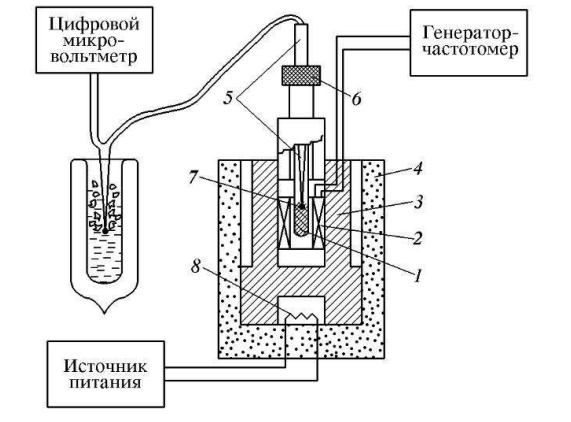
\includegraphics[scale=1]{setup}
	\caption{Схема экспериментальной установки: 1 -- капсула с образцом; 2 -- катушка самоиндукции; 3 -- медный цилиндр; 4 -- пенопластовый корпус; 5 -- шток; 6 -- цанговый зажим; 7 -- измерительный спай термопары; 8 -- электронагреватель} 
\end{figure}

Магнитная восприимчивость образца определяется по изменению самоиндукции, происходящему при его введении в катушку. Обозначая через $L$ самоиндукцию катушки с образцом и через $L_0$ -- ее самоиндукцию в отсутствие образца, получим:

$$
	L = \mu \frac{4 \pi n^2 S}{l}, \ L_0 = \frac{4 \pi n^2 S}{l}
$$

где $\mu$ -- магнитная проницаемость образца, $n$ -- число витков катушки, $l$ -- длина катушки, $S$ -- ее сечение. Тогда

$$
	\frac{L - L_0}{L_0} = \frac{\Delta L}{L_0} = \mu - 1
$$

Так как длина образца существенно больше его диаметра, то размагничивающим фактором можно пренебречь, и выражение оказывается равным:

$$
	\frac{L - L_0}{L_0} = \mu - 1 = 4 \pi \varkappa
$$

\newpage

Учитывая, что частота колебаний $f$ колебательного $LC$-контура определяется выражением $1/f = 2 \pi \sqrt{LC}$, получим

$$
	\frac{f_0^2 - f^2}{f^2} = 4 \pi \varkappa
$$

Отсюда следует, что

$$
	\frac{1}{\varkappa} \propto \frac{f^2}{f_0^2 - f^2}
$$

Разность температур образца и комнаты определяется по показаниям термопары -- $U$ -- с постоянной термопары равной $\alpha = 41 \cdot 10^6 $ В/К

\section*{Ход работы}

Исследуем зависимость частот $f$ и $f_0$ от температуры, постепенно нагревая образец, учитывая что комнатная температура $T_0 = 297 K$. Данные занесем в Таблицы 1,2


\begin{table}[h!]
\centering
\caption{Зависимость собственной частоты колебаний контура с образцом и без от показаний термопары}
\begin{tabular}{|c|c|c|c|c|c|c|c|}
\hline
$U$, мВ & 0,03 & -0,67 & -0,54 & -0,40 & -0,31 & -0,19 & -0,07 \\ \hline
$T$, K & 297,73 & 280,66 & 283,83 & 287,24 & 289,44 & 292,37 & 295,29 \\ \hline
$\sigma_T$, К & 1,03 & 1,03 & 1,03 & 1,03 & 1,03 & 1,03 & 1,03 \\ \hline
$f_0$, кГц & 852,40 & 852,50 & 852,10 & 852,40 & 852,20 & 852,20 & 852,60 \\ \hline
$f$, кГц & 841,00 & 812,10 & 811,70 & 812,20 & 813,20 & 820,60 & 837,20 \\ \hline
$\frac{f^2}{f_0^2 - f^2}$  & 36,64 & 9,81 & 9,80 & 9,86 & 10,18 & 12,74 & 26,93 \\ \hline
$\sigma_{\frac{f^2}{f_0^2 - f^2}}$ & 0,37 & 0,06 & 0,06 & 0,06 & 0,06 & 0,08 & 0,22 \\ \hline
\end{tabular}
\end{table}


\begin{table}[h!]
\centering
\caption{Зависимость собственной частоты колебаний контура с образцом и без от показаний термопары}
\begin{tabular}{|c|c|c|c|c|c|c|c|}
\hline
$U$, мВ & 0,05 & 0,17 & 0,29 & 0,41 & 0,53 & 0,65 & 0,77 \\ \hline
$T$, K & 298,22 & 301,15 & 304,07 & 307,00 & 309,93 & 312,85 & 315,78 \\ \hline
$\sigma_T$, К & 1,03 & 1,03 & 1,03 & 1,03 & 1,03 & 1,03 & 1,03 \\ \hline
$f_0$, кГц & 852,80 & 852,60 & 852,60 & 852,80 & 852,70 & 852,80 & 852,80 \\ \hline
$f$, кГц & 844,80 & 848,30 & 849,60 & 849,90 & 850,50 & 850,70 & 851,00 \\ \hline
$\frac{f^2}{f_0^2 - f^2}$ & 52,55 & 98,39 & 141,35 & 146,28 & 193,05 & 202,30 & 236,14 \\ \hline
$\sigma_{\frac{f^2}{f_0^2 - f^2}}$ & 0,71 & 2,35 & 4,79 & 5,12 & 8,86 & 9,72 & 13,21 \\ \hline
\end{tabular}
\end{table}

где погрешности рассчитывались по формулам

\begin{align*}
	\sigma_{T_0} &= 1 K \\
	\sigma_U &= 0,01 мВ \\ 
	\sigma_T &= \sqrt{\frac{\sigma_U}{\alpha} + \sigma_{T_0}} \approx 1,03 K \\
	\sigma_f &= \sigma_{f_0} = 0,1 кГц \\
	\sigma_{\frac{f^2}{f_0^2 - f^2}} &= \sqrt{ \left( \frac{2f}{f_0^2 - f^2} + \frac{2 f^3}{(f_0^2 - f^2)^2} \right)^2 \sigma_f^2 + \frac{2 f^2 f_0}{(f_0^2 - f^2)^2} \sigma_{f_0}}
\end{align*}

\newpage

По полученным данным построим график зависимости 

\begin{figure}[h!]
	\centering
	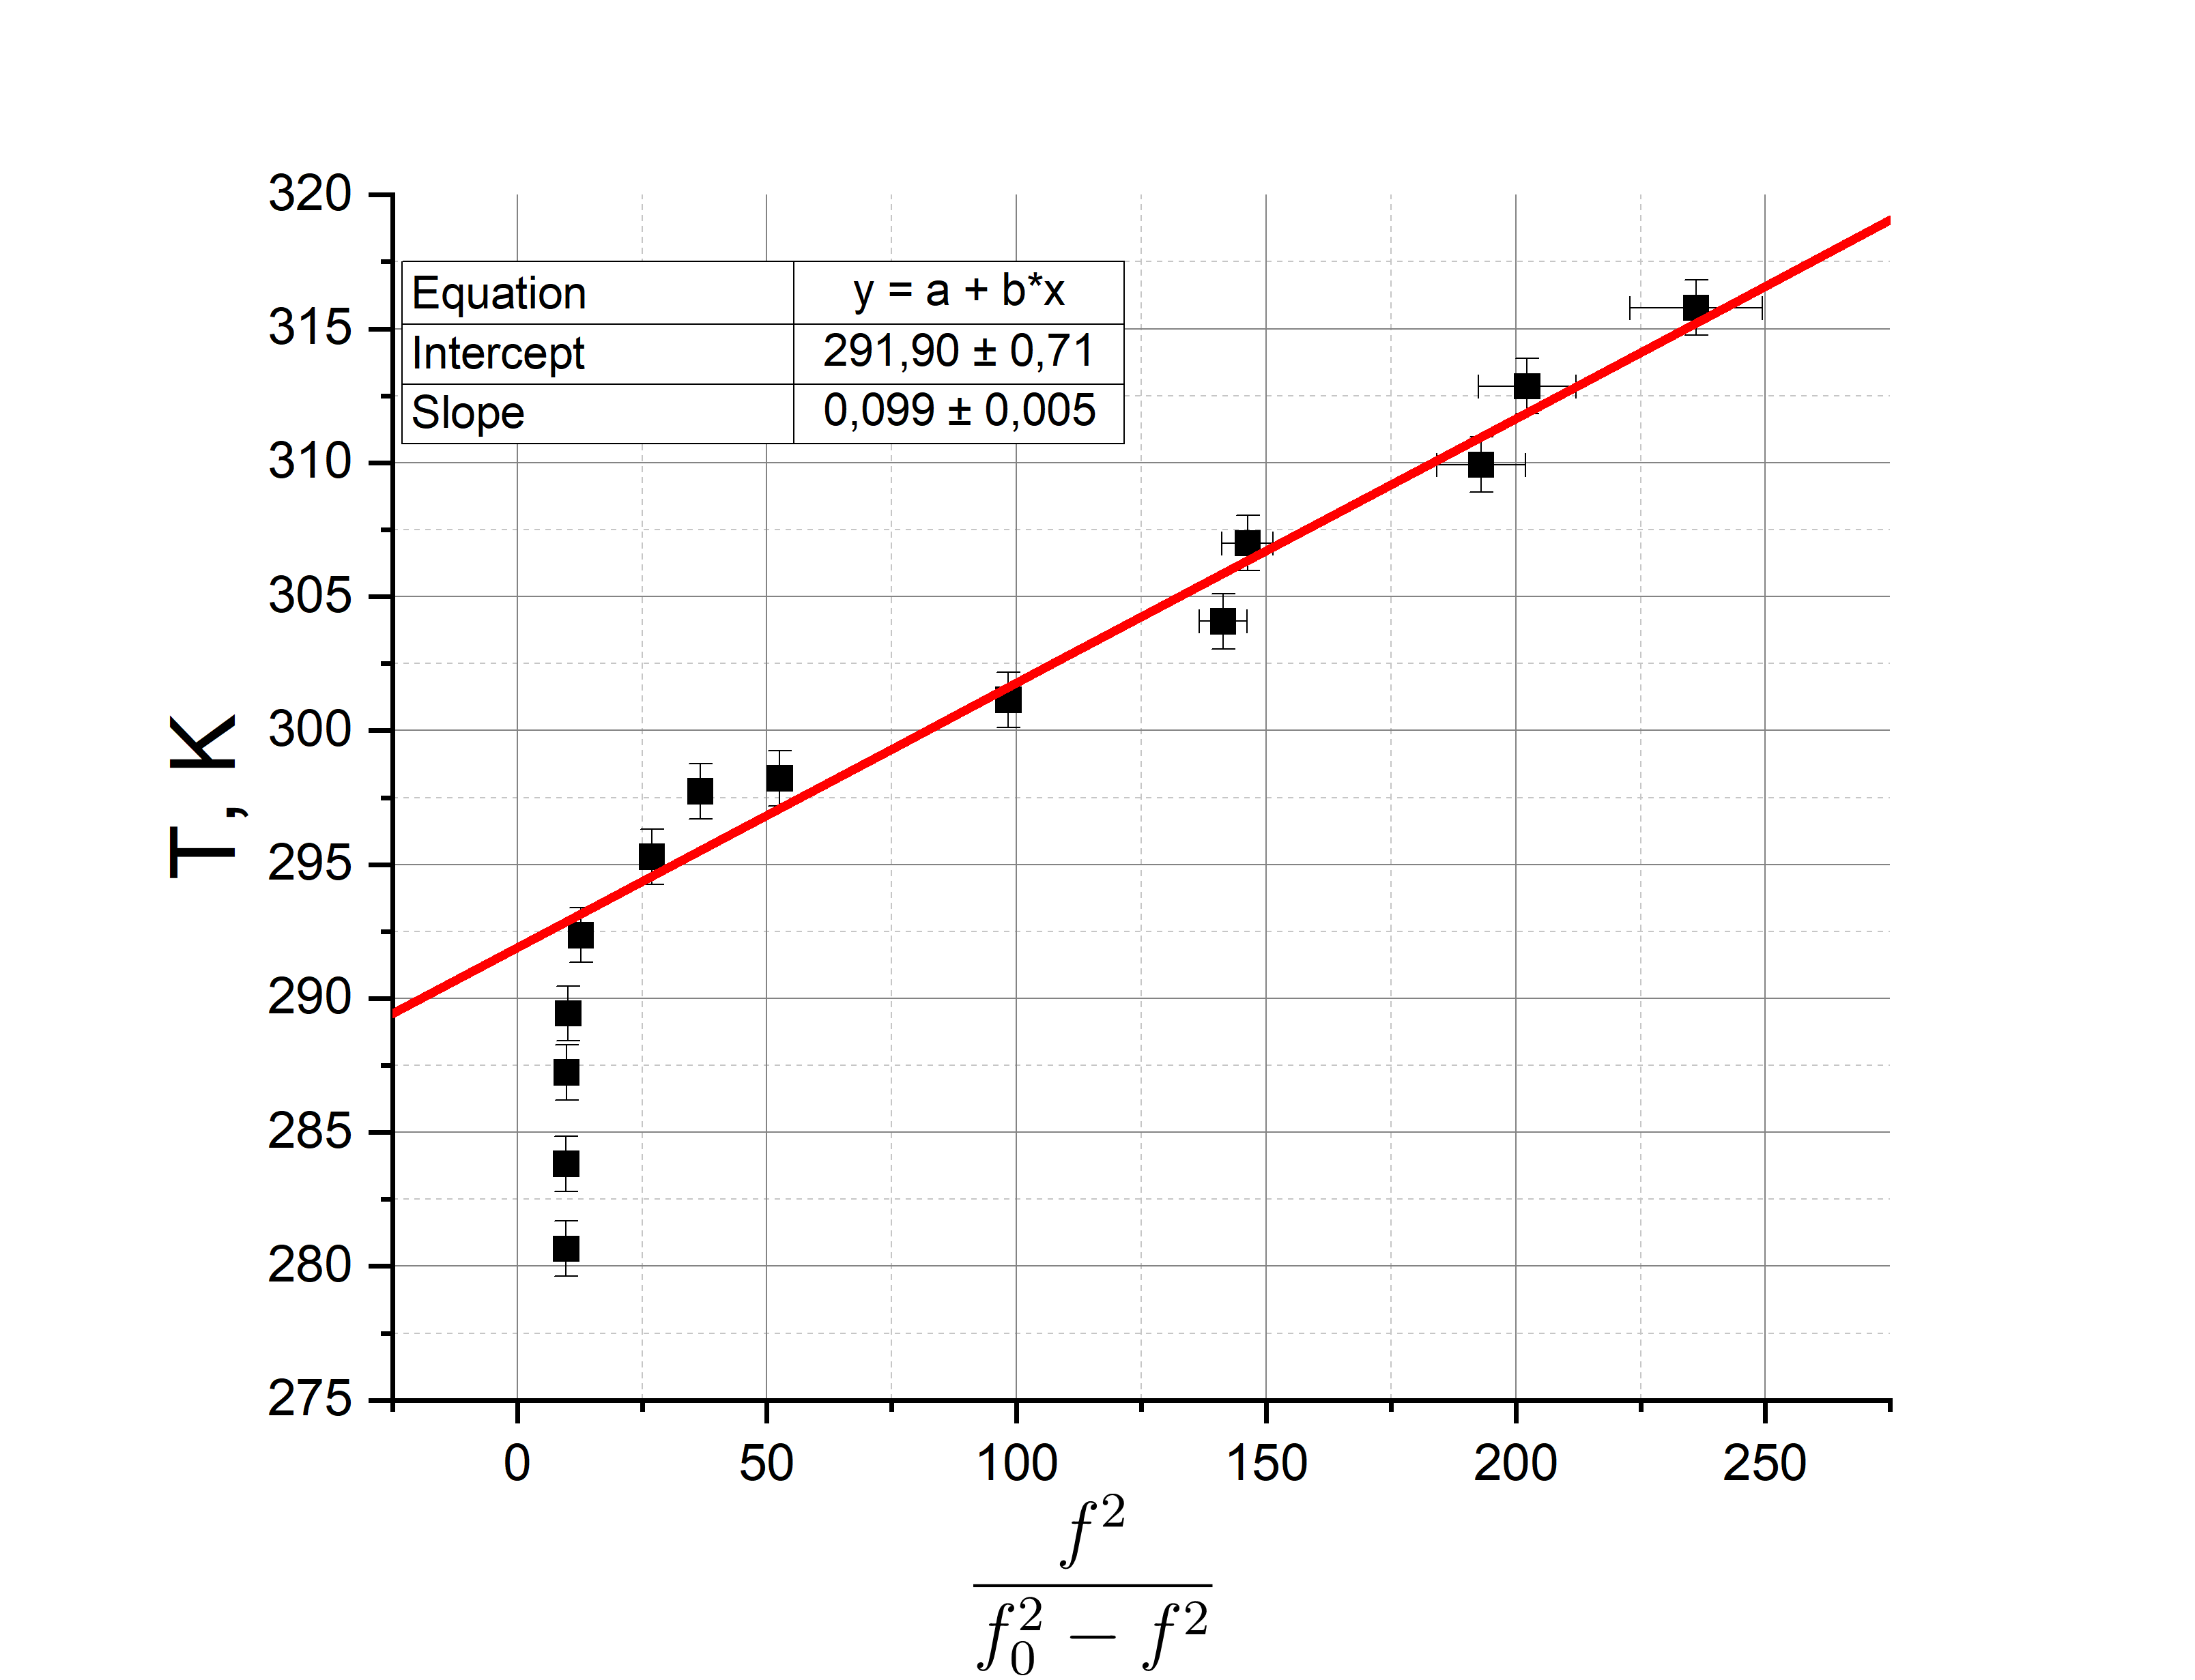
\includegraphics[width = \linewidth]{graph_1}
	\caption{Зависимость $T = g(\frac{f^2}{f_0^2 - f^2})$}
\end{figure}

По методу хи-квадрат приблизим зависимость линейной. Из пересечения линейной зависимости получаем, что температура Кюри для нашего образца:

\begin{align*}
	\Theta = (291,90 \pm 0,71) К 
\end{align*}

По формуле (\ref{obm_int}) оценим величину обменного интеграла, учитывая что для гадолиния $n = 12$ и $J = S = 7/2$:

$$
	J = (199,47 \pm 0,49) мкЭв = (2,317 \pm 0,006) К
$$

где погрешность рассчитывалась по формуле:

$$
	\sigma_J = J \frac{\sigma_{\Theta}}{\Theta}
$$

\newpage

\subsection*{Наблюдение доменной структуры}

В качестве дополнения к работе представим наблюдения доменной структуры ферромагнетика при увеличении прикладываемого магнитного поля	

\begin{figure}[h!]
\centering
\begin{subfigure}{.5\textwidth}
  \centering
  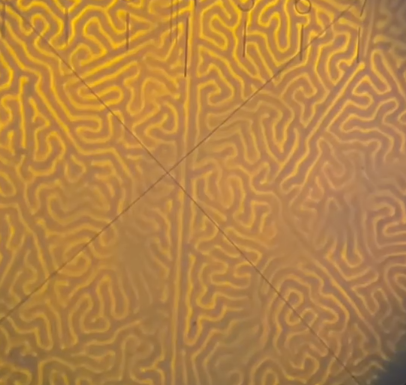
\includegraphics[width=0.8\linewidth]{domen_0}
  \caption{Доменная структура при нулевом \\ магнитном поле}
\end{subfigure}%
\begin{subfigure}{.5\textwidth}
  \centering
  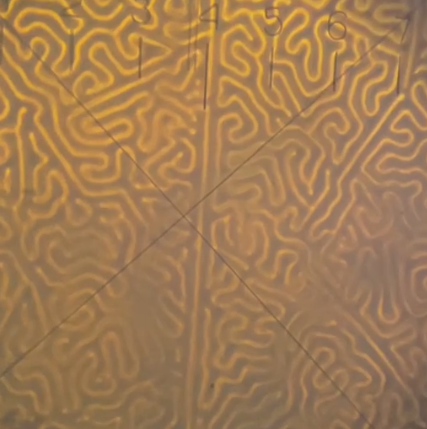
\includegraphics[width=0.8\linewidth]{domen_1}
  \caption{Доменная структура  при величине \\ магнитного поля -- $H_1$}
\end{subfigure}
\end{figure}

\begin{figure}[h!]
\centering
\begin{subfigure}{.5\textwidth}
  \centering
  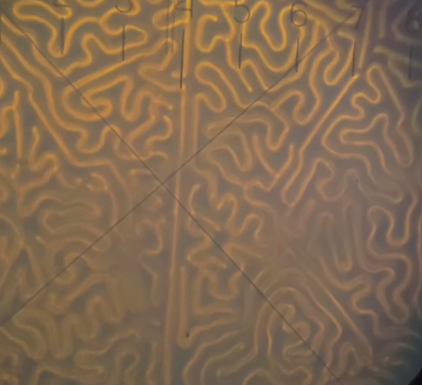
\includegraphics[width=0.8\linewidth]{domen_2}
  \caption{Доменная структура при величине \\ магнитного поля -- $H_2 > H_1$}
\end{subfigure}%
\begin{subfigure}{.5\textwidth}
  \centering
  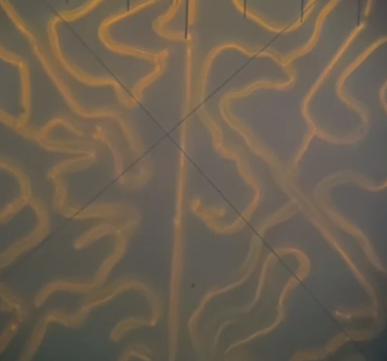
\includegraphics[width=0.8\linewidth]{domen_3}
  \caption{Доменная структура при величине \\ магнитного поля $H_3 > H_2$}
\end{subfigure}
\end{figure}


\section*{Выводы}

\begin{itemize}

\item В результате работы была получена температура Кюри гадолиния  \linebreak $\Theta = ( 291,90 \pm 0,71) K$, что, в пределах погрешности, совпадает с табличным результатом $T_c = 292 K$

\item Было оценено значение обменного интеграла $J \approx (199,47 \pm 0,49) мкЭв = (2,317 \pm \pm 0,006) K$

\item Также, были получены качественные наблюдения изменения доменной структуры ферромагнетика при увеличении внешнего поля 

\end{itemize}

\end{document}